\documentclass[11pt]{article}

\usepackage[margin=1in]{geometry}
\usepackage[T1]{fontenc}
\usepackage{lmodern}
\usepackage{microtype}
\usepackage{amsmath,amssymb,amsthm,mathtools}
\usepackage{mathrsfs}
\usepackage[dvipsnames]{xcolor}
\usepackage[most]{tcolorbox}
\usepackage{tikz}
\usetikzlibrary{decorations.markings,patterns}
\usepackage{enumitem}
\usepackage{tocloft}
\usepackage[hidelinks]{hyperref}

\definecolor{courseblue}{HTML}{1F4E79}
\definecolor{lightblue}{HTML}{EAF2F8}
\definecolor{lightgreen}{HTML}{EAF7EA}
\definecolor{lightpink}{HTML}{FCE8EF}
\definecolor{lightyellow}{HTML}{FFF8D6}
\definecolor{warningyellow}{HTML}{D6A000}
\definecolor{exercisebg}{HTML}{FDEAEA}
\definecolor{exerciseframe}{HTML}{B54040}
\definecolor{examplebg}{HTML}{F4FAFE}
\definecolor{exampleframe}{HTML}{85C1E9}
\definecolor{darkgray}{HTML}{333333}
\definecolor{lightorange}{HTML}{FDEBD8}
\definecolor{orangeframe}{HTML}{E08A3C}

\setlength{\parindent}{0pt}
\setlength{\parskip}{0.65em}
\setlist[itemize]{topsep=0.25em,itemsep=0.15em}
\renewcommand{\cftsecleader}{\cftdotfill{\cftdotsep}}
\renewcommand{\cftsubsecleader}{\cftdotfill{\cftdotsep}}

\theoremstyle{plain}
\newtheorem{theorem}{Theorem}[section]
\newtheorem{proposition}[theorem]{Proposition}
\newtheorem{lemma}[theorem]{Lemma}
\newtheorem{corollary}[theorem]{Corollary}
\theoremstyle{definition}
\newtheorem{definition}[theorem]{Definition}
\newtheorem{example}[theorem]{Example}
\newtheorem{exercise}[theorem]{Exercise}
\theoremstyle{remark}
\newtheorem*{remark}{Remark}
\newtheorem*{fact}{Fact}
\newtheorem*{warning}{Warning}

\tcolorboxenvironment{definition}{
  enhanced,
  unbreakable,
  colback=lightgreen,
  colframe=ForestGreen,
  boxrule=0.7pt,
  arc=2pt,
  left=6pt,
  right=6pt,
  top=5pt,
  bottom=5pt
}

\tcolorboxenvironment{warning}{
  enhanced,
  colback=lightyellow,
  colframe=warningyellow,
  boxrule=0.7pt,
  arc=2pt,
  left=6pt,
  right=6pt,
  top=5pt,
  bottom=5pt
}

\tcolorboxenvironment{exercise}{
  enhanced,
  colback=exercisebg,
  colframe=exerciseframe,
  boxrule=1pt,
  arc=2pt,
  left=6pt,
  right=6pt,
  top=5pt,
  bottom=5pt
}

\tcolorboxenvironment{example}{
  enhanced,
  colback=examplebg,
  colframe=exampleframe,
  boxrule=0.7pt,
  arc=2pt,
  left=6pt,
  right=6pt,
  top=5pt,
  bottom=5pt
}

\numberwithin{equation}{section}

\newcommand{\be}{\begin{eqnarray}}
\newcommand{\ee}{\end{eqnarray}}
\newcommand{\C}{\mathbb{C}}
\newcommand{\R}{\mathbb{R}}
\newcommand{\N}{\mathbb{N}}

\DeclareMathOperator{\Hol}{\mathcal{H}\mathrm{ol}}
\DeclareMathOperator{\Real}{Re}
\DeclareMathOperator{\Imag}{Im}
\newcommand{\A}{\mathcal{A}}
\newcommand{\CT}{\C[[T]]}
\newcommand{\CLT}{\C((T))}
\tcbset{breakable}
\begin{document}

\begin{center}
  \colorbox{lightblue}{%
    \begin{minipage}{0.94\textwidth}
      \vspace{0.55em}
      \begin{tabular*}{\textwidth}{@{\extracolsep{\fill}}lr}
        {\color{courseblue}\bfseries\LARGE Lecture 17} &
        {\color{courseblue}\bfseries\LARGE MATH 411}\\[0.35em]
        \textbf{Fall 2026} & \textbf{Date: Oct 19, 2026}\\
        & \textbf{Instructor: Manish Patnaik}
      \end{tabular*}
      \vspace{0.45em}
    \end{minipage}}
\end{center}

\setcounter{tocdepth}{1}
\tableofcontents
\vspace{0.45em}

% Sources: Lecture 16 (current course), Section 3; handwritten Lecture 16,
% pages 5--7, and handwritten Lecture 17, pages 1--7.
% The overlap-constant argument expands the telescoping step on handwritten
% Lecture 17, pages 4--5. The closed-curve proof and explicit circle homotopy
% supply the contour-deformation justification promised in current Lecture 16.
% Main exposition and redrawn figures follow handwritten Lecture 17 in order:
% definitions (pp. 1--2), theorem and puncture (pp. 2--3), close curves
% (pp. 3--5), homotopy grid (pp. 5--6), horizontal slices (p. 7).
We begin with the definition of homotopy from Lecture~16, then prove that
integrals of holomorphic functions are unchanged by homotopy. Throughout,
$U\subseteq\C$ is open and $a<b$. Integrals along continuous curves have
the meaning defined in Lecture~16, using local primitives on discs.

\section{Homotopy of curves}
\subsection{Homotopy with fixed endpoints}
\begin{definition}\label{def:homotopy}
Let $\gamma,\eta\colon[a,b]\to U$ be continuous curves with
$\gamma(a)=\eta(a)$ and $\gamma(b)=\eta(b)$.
A \emph{homotopy with fixed endpoints} from $\gamma$ to $\eta$ in $U$
is a continuous map
\[
 H\colon[a,b]\times[0,1]\longrightarrow U
\]
such that
\begin{align*}
 H(t,0)&=\gamma(t),&H(t,1)&=\eta(t)&& (a\leq t\leq b),\\
 H(a,s)&=\gamma(a)=\eta(a),&H(b,s)&=\gamma(b)=\eta(b)&& (0\leq s\leq1).
\end{align*}
We write $\gamma\sim\eta$ in $U$ when such a homotopy exists.
\end{definition}
For fixed $s$, write $H_s(t)=H(t,s)$. Thus $H_0=\gamma$,
$H_1=\eta$, and every intermediate curve has the same endpoints.
The parameter $t$ moves along a curve; the parameter $s$ deforms the curve.
The two endpoint conditions hold for every $s$, not just at $s=0$ and $s=1$.

\begin{center}
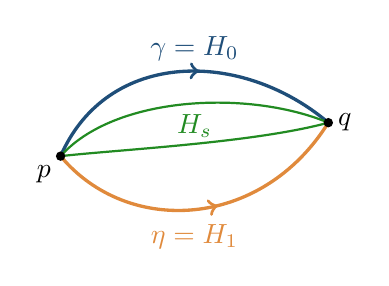
\begin{tikzpicture}[scale=0.85,
 decoration={markings,mark=at position 0.55 with {\arrow{>}}}]
 \draw[very thick,courseblue,postaction={decorate}] (0,0)
 .. controls (0.7,1.6) and (2.7,1.6) .. (4,0.5);
 \draw[very thick,orangeframe,postaction={decorate}] (0,0)
 .. controls (1,-1.2) and (3,-1.1) .. (4,0.5);
 \draw[ForestGreen,thick] (0,0) .. controls (0.8,0.9) and (2.8,1) .. (4,0.5);
 \draw[ForestGreen,thick] (0,0) .. controls (0.9,0.1) and (2.9,0.2) .. (4,0.5);
 \fill (0,0) circle (2pt) node[below left]{$p$};
 \fill (4,0.5) circle (2pt) node[right]{$q$};
 \node[courseblue] at (2,1.6){$\gamma=H_0$};
 \node[orangeframe] at (2,-1.2){$\eta=H_1$};
 \node[ForestGreen] at (2,0.45){$H_s$};
\end{tikzpicture}
\end{center}

\begin{example}[Straight-line homotopy]
Recall that $U$ is convex if it contains the line segment joining any
two of its points. If $U$ is convex and $\gamma,\eta$ have the same
endpoints, then
\[
 H(t,s)=(1-s)\gamma(t)+s\eta(t)
\]
is a homotopy with fixed endpoints in $U$. Indeed, it is continuous,
convexity keeps its values in $U$, and the boundary conditions hold.
\end{example}

\subsection{Closed curves and simple connectivity}
\begin{definition}\label{def:closed-homotopy}
Two closed continuous curves $\gamma,\eta\colon[a,b]\to U$ are
\emph{homotopic through closed curves in $U$} if there is a continuous
map $H\colon[a,b]\times[0,1]\to U$ such that
\[
 H(t,0)=\gamma(t),\qquad H(t,1)=\eta(t),\qquad
 H(a,s)=H(b,s).
\]
These identities hold for all $t\in[a,b]$ and $s\in[0,1]$.
The common start and end point may move as $s$ varies.
\end{definition}
This differs from homotopy with fixed endpoints: the last condition
requires each intermediate curve to be closed, but does not fix its base point.

\begin{definition}
A closed curve $\gamma$ in $U$ is \emph{null-homotopic in $U$} if it
is homotopic through closed curves to a constant curve $c_p(t)=p$,
for some $p\in U$.
A nonempty open connected set $U$ is \emph{simply connected} if every closed
continuous curve in $U$ is null-homotopic in $U$.
\end{definition}
For a nonempty convex open set, the homotopy
$H(t,s)=(1-s)\gamma(t)+sp$ contracts any closed curve to a point
$p\in U$. Thus every such set is simply connected.
The ambient set matters: a deformation must stay in $U$ at every stage.

% Redrawn from handwritten Lecture 17, page 2.
\begin{center}
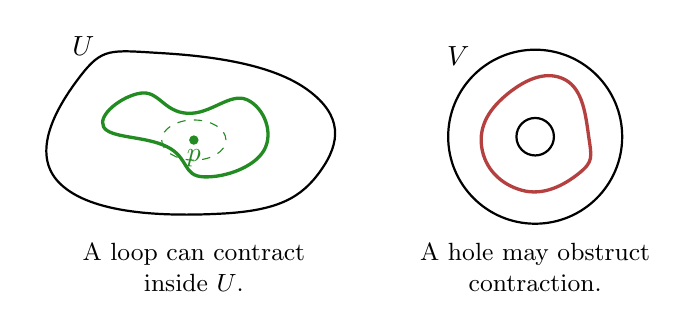
\begin{tikzpicture}[scale=0.85]
 \draw[thick] plot[smooth cycle,tension=0.8] coordinates
 {(-2,-0.7) (-1.7,0.9) (-0.5,1.25) (1.7,0.7) (1.9,-0.5) (0.4,-1.15)};
 \draw[ForestGreen,very thick] plot[smooth cycle,tension=0.8] coordinates
 {(-1.35,0.15) (-0.8,0.65) (-0.1,0.35) (0.8,0.55) (1.05,-0.2) (0.15,-0.6) (-0.4,-0.15)};
 \draw[ForestGreen,dashed] (0,-0.05) ellipse (0.48 and 0.3);
 \fill[ForestGreen] (0,-0.05) circle (2pt) node[below]{$p$};
 \node at (-1.65,1.35){$U$};
 \node[below,font=\small,align=center] at (0,-1.45){A loop can contract\\inside $U$.};
 \begin{scope}[xshift=5.1cm]
  \draw[thick] (0,0) circle (1.3);
  \fill[white] (0,0) circle (0.28);
  \draw[thick] (0,0) circle (0.28);
  \draw[exerciseframe,very thick] plot[smooth cycle,tension=0.8] coordinates
  {(0.8,0) (0.45,0.85) (-0.4,0.65) (-0.8,-0.15) (-0.2,-0.8) (0.65,-0.55)};
  \node at (-1.15,1.2){$V$};
  \node[below,font=\small,align=center] at (0,-1.45){A hole may obstruct\\contraction.};
 \end{scope}
\end{tikzpicture}
\end{center}
The right-hand picture suggests an obstruction; the example below will
prove it for a punctured disc by integrating $1/z$.


\newpage
\section{The homotopy form of Cauchy's theorem}
\begin{theorem}[Homotopy form of Cauchy's theorem]\label{thm:homotopy}
Let $f$ be holomorphic on an open set $U\subseteq\C$, and let
$\gamma,\eta\colon[a,b]\to U$ be continuous curves.
If $\gamma$ and $\eta$ are homotopic with fixed endpoints in $U$, then
\begin{equation}\label{eq:homotopy-invariance}
 \boxed{\displaystyle\int_\gamma f(z)\,dz=\int_\eta f(z)\,dz.}
\end{equation}
The same conclusion holds if $\gamma$ and $\eta$ are closed and
homotopic through closed curves in $U$.
\end{theorem}

\begin{example}[A puncture prevents contraction]
Let $U=\{z\in\C:0<|z|<1\}$ and $0<r<1$. For the circle
$C_r(t)=re^{it}$, $0\leq t\leq2\pi$,
\[
 \int_{C_r}\frac{dz}{z}
 =\int_0^{2\pi}\frac{ire^{it}}{re^{it}}\,dt=2\pi i.
\]
Since $1/z$ is holomorphic on $U$, Theorem~\ref{thm:homotopy} shows that
$C_r$ is not null-homotopic in $U$. Indeed, a contraction would force this integral to equal the integral
over a constant curve, which is zero. Thus $U$ is not simply connected.
For any $0<\rho<1$, the circles $C_r,C_\rho$ are homotopic through
closed curves in $U$ via
\[
 H(t,s)=\bigl((1-s)r+s\rho\bigr)e^{it},
\]
and their integrals agree. A homotopy to a constant curve guarantees
vanishing; it is not necessary for a particular integrand. For example,
$\int_{C_r}1\,dz=0$, although $C_r$ is not null-homotopic in $U$.

% Redrawn from handwritten Lecture 17, page 3.
\begin{center}
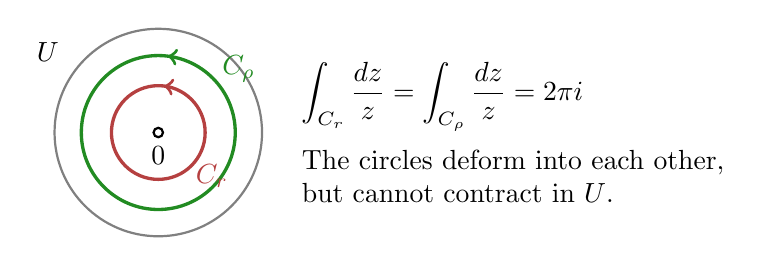
\begin{tikzpicture}[scale=0.85,
 decoration={markings,mark=at position 0.23 with {\arrow{>}}}]
 \draw[gray,thick] (0,0) circle (1.55);
 \draw[exerciseframe,very thick,postaction={decorate}] (0.7,0)
 arc[start angle=0,end angle=360,radius=0.7];
 \draw[ForestGreen,very thick,postaction={decorate}] (1.15,0)
 arc[start angle=0,end angle=360,radius=1.15];
 \draw[fill=white,thick] (0,0) circle (2pt);
 \node[below] at (0,-0.06){$0$};
 \node[exerciseframe] at (0.8,-0.65){$C_r$};
 \node[ForestGreen] at (1.2,0.95){$C_\rho$};
 \node at (-1.65,1.2){$U$};
 \node[right,align=left] at (2,0)
 {$\displaystyle\int_{C_r}\frac{dz}{z}=\int_{C_\rho}\frac{dz}{z}=2\pi i$\\[0.6em]
  The circles deform into each other,\\but cannot contract in $U$.};
\end{tikzpicture}
\end{center}

\end{example}

\textbf{Proof strategy.} We first compare
curves that are close in the sense that corresponding pieces lie in the
same discs. We then use compactness and uniform continuity to subdivide
a homotopy into finitely many such comparisons.
No differentiability of the homotopy or its intermediate curves is required.

% Local comparison sketch from handwritten Lecture 17, page 3.
\begin{center}
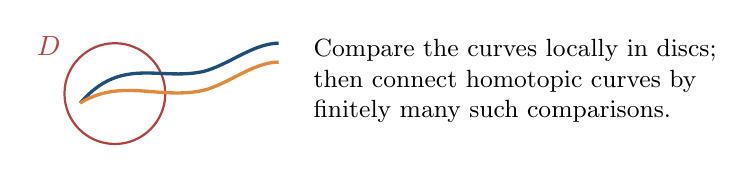
\begin{tikzpicture}[scale=0.8]
 \draw[exerciseframe,thick] (0,0) circle (0.8);
 \draw[very thick,courseblue] (-0.55,-0.15)
 .. controls (0.1,0.6) and (0.7,0.2) .. (1.4,0.35)
 .. controls (1.8,0.45) and (2.2,0.8) .. (2.6,0.8);
 \draw[very thick,orangeframe] (-0.55,-0.15)
 .. controls (0.1,0.25) and (0.7,-0.1) .. (1.4,0.05)
 .. controls (1.8,0.15) and (2.2,0.5) .. (2.6,0.5);
 \node[exerciseframe] at (-1.05,0.75){$D$};
 \node[right,align=left,font=\small] at (3,0.2)
 {Compare the curves locally in discs;\\then connect homotopic curves by\\finitely many such comparisons.};
\end{tikzpicture}
\end{center}


\subsection{Step 1: curves in a common chain of discs}
\begin{definition}[Close curves]\label{def:close}
Two continuous curves $\alpha,\beta\colon[a,b]\to U$ with the same
endpoints are called \emph{close} if there exist a subdivision
\[
 a=t_0<t_1<\cdots<t_n=b
\]
and open discs $D_0,\ldots,D_{n-1}\subseteq U$ such that, for every $j$,
\[
 \alpha([t_j,t_{j+1}])\cup\beta([t_j,t_{j+1}])\subseteq D_j.
\]
Thus the same subdivision and the same discs form a partition of both curves.
\end{definition}

\begin{center}
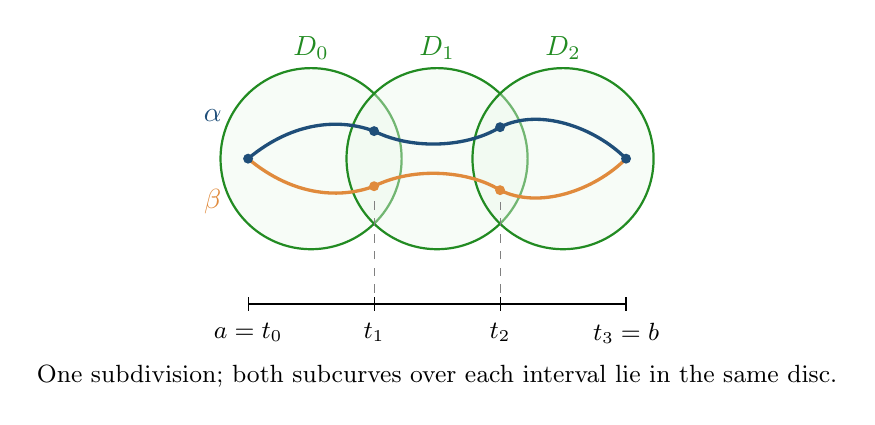
\begin{tikzpicture}[x=1cm,y=1cm]
 \foreach \x in {0,1.6,3.2} {
  \fill[lightgreen,opacity=0.4] (\x,0) circle (1.15);
  \draw[ForestGreen,thick] (\x,0) circle (1.15);
 }
 \draw[very thick,courseblue] (-0.8,0)
 .. controls (-0.2,0.5) and (0.4,0.5) .. (0.8,0.35)
 .. controls (1.3,0.1) and (2,0.15) .. (2.4,0.4)
 .. controls (2.9,0.65) and (3.6,0.4) .. (4,0);
 \draw[very thick,orangeframe] (-0.8,0)
 .. controls (-0.2,-0.5) and (0.4,-0.5) .. (0.8,-0.35)
 .. controls (1.3,-0.1) and (2,-0.15) .. (2.4,-0.4)
 .. controls (2.9,-0.65) and (3.6,-0.4) .. (4,0);
 \foreach \x/\y in {-0.8/0,0.8/0.35,2.4/0.4,4/0}
  {\fill[courseblue] (\x,\y) circle (1.8pt);}
 \foreach \x/\y in {0.8/-0.35,2.4/-0.4}
  {\fill[orangeframe] (\x,\y) circle (1.8pt);}
 \node[ForestGreen] at (0,1.4){$D_0$};
 \node[ForestGreen] at (1.6,1.4){$D_1$};
 \node[ForestGreen] at (3.2,1.4){$D_2$};
 \node[courseblue] at (-1.25,0.55){$\alpha$};
 \node[orangeframe] at (-1.25,-0.55){$\beta$};
 \draw[thick] (-0.8,-1.85)--(4,-1.85);
 \foreach \x/\lab in {-0.8/{a=t_0},0.8/{t_1},2.4/{t_2},4/{t_3=b}} {
  \draw (\x,-1.76)--(\x,-1.94);
  \node[below,font=\small] at (\x,-1.97){$\lab$};
 }
 \draw[gray,dashed] (0.8,-1.7)--(0.8,-0.5);
 \draw[gray,dashed] (2.4,-1.7)--(2.4,-0.55);
 \node[below,font=\small] at (1.6,-2.5)
 {One subdivision; both subcurves over each interval lie in the same disc.};
\end{tikzpicture}
\end{center}

\begin{lemma}\label{lem:close}
If $\alpha$ and $\beta$ are close and $f$ is holomorphic on $U$, then
$\int_\alpha f(z)\,dz=\int_\beta f(z)\,dz$.
\end{lemma}
\begin{proof}
Choose a primitive $g_j$ of $f$ on each $D_j$, using Cauchy's theorem
on a disc. By the definition of
integration along continuous curves,
\begin{align*}
 \int_\alpha f(z)\,dz
 &=\sum_{j=0}^{n-1}\bigl[g_j(\alpha(t_{j+1}))-g_j(\alpha(t_j))\bigr],\\
 \int_\beta f(z)\,dz
 &=\sum_{j=0}^{n-1}\bigl[g_j(\beta(t_{j+1}))-g_j(\beta(t_j))\bigr].
\end{align*}
For $t\in[t_j,t_{j+1}]$, put
\[
 A_j(t)=g_j(\alpha(t))-g_j(\beta(t)).
\]
Subtracting the two integral formulas gives
\begin{equation}\label{eq:close-difference}
 \int_\alpha f(z)\,dz-\int_\beta f(z)\,dz
 =\sum_{j=0}^{n-1}\bigl[A_j(t_{j+1})-A_j(t_j)\bigr].
\end{equation}

\pagebreak[3]
\textbf{Why do the interior terms cancel?}
For $1\leq j\leq n-1$, both $\alpha(t_j)$ and $\beta(t_j)$ lie in
$D_{j-1}\cap D_j$. This intersection is nonempty and convex, hence
connected. Since
\[
 (g_{j-1}-g_j)'=f-f=0,
\]
we have $g_{j-1}-g_j=C_j$ on this intersection. Consequently,
\begin{align*}
 A_{j-1}(t_j)
 &=\bigl[g_j(\alpha(t_j))+C_j\bigr]
   -\bigl[g_j(\beta(t_j))+C_j\bigr]\\
 &=A_j(t_j).
\end{align*}
Thus \eqref{eq:close-difference} becomes
\[
 A_{n-1}(b)-A_0(a)
 +\sum_{j=1}^{n-1}\underbrace{\bigl[A_{j-1}(t_j)-A_j(t_j)\bigr]}_{0}.
\]
The remaining endpoint terms vanish because $\alpha(a)=\beta(a)$ and
$\alpha(b)=\beta(b)$. This proves the lemma.
\end{proof}

\begin{remark}
The primitives $g_{j-1}$ and $g_j$ need not agree on an overlap.
Their difference is constant there, which is precisely what makes the
\emph{differences of endpoint values} agree and the sum telescope.
\end{remark}

\subsection{Step 2: subdividing the homotopy}

We have proved the local comparison. To compare homotopic curves, we
now seek finitely many levels $0=s_0<\cdots<s_m=1$ such that
$H(\cdot,s_k)$ and $H(\cdot,s_{k+1})$ are close for every $k$.
The picture suggests subdividing the parameter rectangle in both directions.

% Redrawn from handwritten Lecture 17, page 5: a family of curves,
% a small disc around pieces of that family, and the parameter grid.
\begin{center}
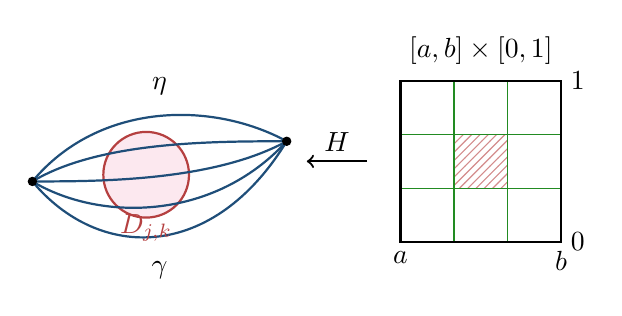
\begin{tikzpicture}[scale=0.85]
 \fill[lightpink] (1.7,0.1) circle (0.64);
 \draw[exerciseframe,thick] (1.7,0.1) circle (0.64);
 \foreach \h in {-1.2,-0.6,0,0.6,1.2} {
  \draw[courseblue,thick] (0,0)
   .. controls (1,\h) and (2.7,\h) .. (3.8,0.6);
 }
 \fill (0,0) circle (2pt); \fill (3.8,0.6) circle (2pt);
 \node[above] at (1.9,1.15){$\eta$};
 \node[below] at (1.9,-1.05){$\gamma$};
 \node[exerciseframe] at (1.7,-0.7){$D_{j,k}$};
 \draw[->,thick] (5,0.3)--(4.1,0.3) node[midway,above]{$H$};
 \begin{scope}[xshift=5.5cm,yshift=-0.9cm]
  \fill[pattern=north east lines,pattern color=exerciseframe!60]
   (0.8,0.8) rectangle (1.6,1.6);
  \draw[step=0.8,ForestGreen] (0,0) grid (2.4,2.4);
  \draw[thick] (0,0) rectangle (2.4,2.4);
  \node[below] at (0,0){$a$}; \node[below] at (2.4,0){$b$};
  \node[right] at (2.4,0){$0$}; \node[right] at (2.4,2.4){$1$};
  \node[above] at (1.2,2.5){$[a,b]\times[0,1]$};
 \end{scope}
\end{tikzpicture}
\end{center}

\begin{lemma}[A grid of small rectangles]\label{lem:grid}
Let $H\colon[a,b]\times[0,1]\to U$ be continuous. There exist subdivisions
\[
 a=t_0<\cdots<t_n=b,\qquad 0=s_0<\cdots<s_m=1
\]
and open discs $D_{j,k}\subseteq U$ such that, writing
$R_{j,k}=[t_j,t_{j+1}]\times[s_k,s_{k+1}]$,
\[
 H(R_{j,k})\subseteq D_{j,k}
 \quad(0\leq j<n,\ 0\leq k<m).
\]
\end{lemma}
\begin{proof}
\textbf{First choose a radius in the image.}
The image $K=H([a,b]\times[0,1])$ is compact. By the
uniform-neighbourhood lemma from Lecture~15, choose $r>0$ such that
\[
 D(w,r)\subseteq U\qquad\text{for every }w\in K.
\]
\textbf{Then choose a mesh in the parameter rectangle.}
Since $H$ is continuous on a compact rectangle, it is uniformly
continuous. Choose $\delta>0$ such that
\[
 \|(t,s)-(t',s')\|<\delta
 \quad\Longrightarrow\quad
 |H(t,s)-H(t',s')|<r/2.
\]
Choose both subdivisions with all their interval lengths less than
$\delta/2$. Each small rectangle then has diameter less than
$\sqrt{2}\,\delta/2<\delta$. Set
\[
 D_{j,k}=D\bigl(H(t_j,s_k),r\bigr).
\]
Every point $(t,s)$ of the corresponding rectangle satisfies
\[
 |H(t,s)-H(t_j,s_k)|<r/2<r,
\]
so its image lies in $D_{j,k}\subseteq U$, as required.
The radius $r$ and the number $\delta$ work for the entire homotopy,
so one finite grid suffices.
\end{proof}

\begin{center}
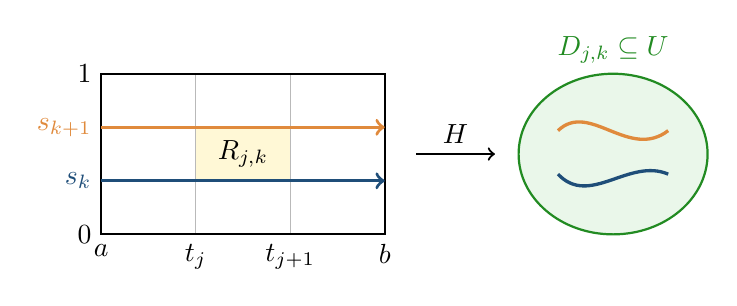
\begin{tikzpicture}[x=1cm,y=0.85cm]
 \fill[lightyellow] (1.2,0.8) rectangle (2.4,1.6);
 \draw[gray!55] (1.2,0)--(1.2,2.4) (2.4,0)--(2.4,2.4);
 \draw[gray!55] (0,0.8)--(3.6,0.8) (0,1.6)--(3.6,1.6);
 \draw[thick] (0,0) rectangle (3.6,2.4);
 \draw[very thick,courseblue,->] (0,0.8)--(3.6,0.8);
 \draw[very thick,orangeframe,->] (0,1.6)--(3.6,1.6);
 \node[left] at (0,0){$0$}; \node[left] at (0,2.4){$1$};
 \node[left,courseblue] at (0,0.8){$s_k$};
 \node[left,orangeframe] at (0,1.6){$s_{k+1}$};
 \node[below] at (0,0){$a$}; \node[below] at (3.6,0){$b$};
 \node[below] at (1.2,0){$t_j$}; \node[below] at (2.4,0){$t_{j+1}$};
 \node at (1.8,1.2){$R_{j,k}$};
 \draw[thick,->] (4,1.2)--(5,1.2) node[midway,above]{$H$};
 \fill[lightgreen] (6.5,1.2) circle (1.2);
 \draw[ForestGreen,thick] (6.5,1.2) circle (1.2);
 \draw[very thick,courseblue] (5.8,0.9)
 .. controls (6.2,0.4) and (6.7,1.15) .. (7.2,0.9);
 \draw[very thick,orangeframe] (5.8,1.55)
 .. controls (6.2,2) and (6.7,1.1) .. (7.2,1.55);
 \node[ForestGreen] at (6.5,2.75){$D_{j,k}\subseteq U$};
\end{tikzpicture}
\end{center}
The image of a small rectangle need not itself be a rectangle, or even
have a simple shape. What matters is that it lies in one disc. In
particular, the two horizontal edges map to curves in the same disc.

\begin{proof}[Proof of Theorem~\ref{thm:homotopy} for fixed endpoints]
Let $H$ be the given homotopy and choose the grid from
Lemma~\ref{lem:grid}. For $0\leq k\leq m$, define
\[
 \gamma_k(t)=H(t,s_k),\qquad a\leq t\leq b.
\]
Then $\gamma_0=\gamma$ and $\gamma_m=\eta$. All these curves have
the same endpoints. For $0\leq j<n$ and $0\leq k<m$,
\[
 \gamma_k([t_j,t_{j+1}])\cup\gamma_{k+1}([t_j,t_{j+1}])
 \subseteq D_{j,k}.
\]
Thus consecutive curves $\gamma_k$ and $\gamma_{k+1}$ are close.

% Redrawn from handwritten Lecture 17, page 7: the horizontal slices.
\begin{center}
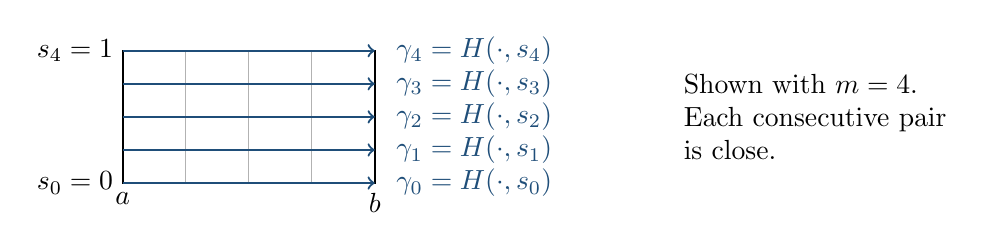
\begin{tikzpicture}[x=1cm,y=0.7cm]
 \draw[gray!60] (0.8,0)--(0.8,2.4) (1.6,0)--(1.6,2.4)
  (2.4,0)--(2.4,2.4);
 \draw[thick] (0,0) rectangle (3.2,2.4);
 \foreach \y/\lab in {0/0,0.6/1,1.2/2,1.8/3,2.4/4} {
  \draw[courseblue,thick,->] (0,\y)--(3.2,\y);
  \node[right,courseblue] at (3.35,\y){$\gamma_{\lab}=H(\cdot,s_{\lab})$};
 }
 \node[left] at (0,0){$s_0=0$};
 \node[left] at (0,2.4){$s_4=1$};
 \node[below] at (0,0){$a$}; \node[below] at (3.2,0){$b$};
 \node[align=left,right] at (7,1.2)
 {Shown with $m=4$.\\Each consecutive pair\\is close.};
\end{tikzpicture}
\end{center}

Lemma~\ref{lem:close} gives
\[
 \int_{\gamma_0}f(z)\,dz
 =\int_{\gamma_1}f(z)\,dz
 =\cdots
 =\int_{\gamma_m}f(z)\,dz,
\]
which is the desired equality.
\end{proof}

\section{Closed-curve version and consequences}
\subsection{Allowing the base point to move}
We now prove the second assertion of the theorem. The moving base point
means we cannot directly use the fixed-endpoint hypothesis of
Lemma~\ref{lem:close}. Instead, we keep track of the two side curves.

\begin{proof}[Proof of Theorem~\ref{thm:homotopy} for closed curves]
Choose a grid for the given closed-curve homotopy as in
Lemma~\ref{lem:grid}, and put $\gamma_k(t)=H(t,s_k)$.
Traverse the boundary of each small rectangle counterclockwise in the
parameter plane. Composing this traversal with $H$ gives a closed
continuous curve in $D_{j,k}$. Since $f$ has a primitive there, its integral
is zero.

Fix a horizontal strip $[a,b]\times[s_k,s_{k+1}]$ and add these zero
integrals over its $n$ rectangles. Every interior vertical edge is
traversed twice in opposite directions, so these contributions cancel.
Write
\[
 L_k(s)=H(a,s),\qquad R_k(s)=H(b,s),\qquad s_k\leq s\leq s_{k+1},
\]
with both side curves parametrized by increasing $s$. The bottom and
right edges are traversed in the positive parameter directions, while
the top and left edges are traversed in reverse. Thus
\[
 0=\int_{\gamma_k}f(z)\,dz+\int_{R_k}f(z)\,dz
   -\int_{\gamma_{k+1}}f(z)\,dz-\int_{L_k}f(z)\,dz.
\]
For a homotopy through closed curves, $H(a,s)=H(b,s)$; hence
$L_k=R_k$ as parametrized curves, and their integrals cancel too.
Therefore $\int_{\gamma_k}f=\int_{\gamma_{k+1}}f$ for every $k$.
Chaining the equalities proves $\int_\gamma f=\int_\eta f$.
\end{proof}

\subsection{Null-homotopic curves}
\begin{corollary}[Cauchy's theorem for a null-homotopic curve]
If $f$ is holomorphic on $U$ and $\gamma$ is a closed continuous curve
that is null-homotopic in $U$, then
\[
 \int_\gamma f(z)\,dz=0.
\]
In particular, if $U$ is simply connected, the integral of every
holomorphic function on $U$ around every closed continuous curve in $U$
is zero.
\end{corollary}
\begin{proof}
Deform $\gamma$ through closed curves to a constant curve. The theorem
preserves the integral, and the integral over a constant curve is zero.
\end{proof}



\newpage
\subsection{Justifying the deformation in Lecture 16}
Let $D=D(c,R)$, let $U$ contain $\overline D$, let $f$ be holomorphic
on $U$, and take $z_0\in D$.
In Lecture~16 we deformed the outer circle $\gamma(t)=c+Re^{it}$ to
$C_r(t)=z_0+re^{it}$, where $0<r<R-|z_0-c|$. An explicit homotopy is
\[
 H(t,s)=(1-s)c+sz_0+\bigl((1-s)R+sr\bigr)e^{it},
 \qquad 0\leq t\leq2\pi,\quad 0\leq s\leq1.
\]
Put $d=|z_0-c|<R$. The estimates
\begin{align*}
 |H(t,s)-c|&\leq sd+(1-s)R+sr\leq R,\\
 |H(t,s)-z_0|&\geq(1-s)(R-d)+sr>0
\end{align*}
show that the deformation stays in $\overline D\setminus\{z_0\}$,
hence in $U\setminus\{z_0\}$. Also $H(0,s)=H(2\pi,s)$.
The closed-curve form of Theorem~\ref{thm:homotopy} therefore gives
\[
 \int_\gamma h(z)\,dz=\int_{C_r}h(z)\,dz
 \qquad\text{for every }h\in\Hol(U\setminus\{z_0\}).
\]
Apply this to $h(z)=(f(z)-f(z_0))/(z-z_0)$ and to $h(z)=1/(z-z_0)$.
These are exactly the two contour-deformation steps used in Lecture~16;
the boundedness estimate and the circle computation there now complete
the proof of the local Cauchy integral formula.

\begin{exercise}
Let $U$ be convex and open, and let $f$ be holomorphic on $U$.
Use straight-line homotopy and Theorem~\ref{thm:homotopy} to show that
$\int_\gamma f(z)\,dz$ depends only on the endpoints of $\gamma$.
Explain why this also proves that the integral is zero on every closed
continuous curve in $U$.
\end{exercise}

\end{document}
